\documentclass[xetex,mathserif,serif]{beamer}
\usepackage{polyglossia}
\setdefaultlanguage[babelshorthands=true]{russian}
\usepackage{minted}
\usepackage{tabu}

\useoutertheme{infolines}

\usepackage{fontspec}
\setmainfont{FreeSans}
\newfontfamily{\russianfonttt}{FreeSans}

\definecolor{links}{HTML}{2A1B81}
\hypersetup{colorlinks,linkcolor=,urlcolor=links}

\setbeamertemplate{blocks}[rounded][shadow=false]

\setbeamercolor*{block title alerted}{fg=red!50!black,bg=red!20}
\setbeamercolor*{block body alerted}{fg=black,bg=red!10}

\tabulinesep=1.2mm

\title{Экосистема open source проектов}
\subtitle{Полезные инструменты и сервисы}
\author[Юрий Литвинов]{Юрий Литвинов\\\small{\textcolor{gray}{y.litvinov@spbu.ru}}}
\date{18.03.2022}

\newcommand{\attribution}[1] {
\vspace{-5mm}\begin{flushright}\begin{scriptsize}\textcolor{gray}{\textcopyright\, #1}\end{scriptsize}\end{flushright}
}

\begin{document}

    \frame{\titlepage}

    \section{CI}

    \subsection{Работа с консолью}

    \begin{frame}
        \frametitle{Небольшое отступление про сборку из консоли}
        \framesubtitle{В Windows, остальные и так умеют}
        \begin{itemize}
            \item Основные консольные команды: cd, dir
            \item Переменные окружения, PATH
            \item .NET SDK
            \item NuGet Command Line
            \item Как сделать жизнь более удобной
            \begin{itemize}
                \item FAR (\url{https://www.farmanager.com/})
                \item Chocolatey (\url{https://chocolatey.org/})
            \end{itemize}
        \end{itemize}
    \end{frame}

    \begin{frame}
        \frametitle{Основные команды .NET Command-Line Interface}
        \begin{itemize}
            \item dotnet new --- создать новый проект
            \begin{itemize}
                \item dotnet new console
            \end{itemize}
            \item dotnet restore --- получить NuGet-пакеты для текущего проекта
            \item dotnet build --- собрать проект в текущей папке
            \item dotnet run --- запустить проект в текущей папке
            \begin{itemize}
                \item \mintinline{text}{dotnet run -- моиАргументы}
            \end{itemize}
            \item dotnet test --- запустить юнит-тесты для проекта в текущей папке
        \end{itemize}
    \end{frame}

    \subsection{Continuous Integration}

    \begin{frame}
        \frametitle{Continuous Integration}
        Непрерывная интеграция --- практика слияния всех изменений по нескольку раз в день, сборки их в известном окружении и запуска юнит-тестов.
        \begin{itemize}
            \item Автоматический билд
            \begin{itemize}
                \item Всё, что нужно для сборки, есть в репозитории, может быть получено на чистую (ну, практически) машину и собрано одной консольной командой
            \end{itemize}
            \item Большое количество юнит-тестов, запускаемых автоматически
            \item Выделенная машина, слушающая репозиторий и выполняющая билд
            \begin{itemize}
                \item Чаще всего каждый билд запускается на заранее настроенной виртуалке
            \end{itemize}
        \end{itemize}
    \end{frame}

    \begin{frame}
        \frametitle{Continuous Integration}
        \begin{itemize}
            \item Извещение всех разработчиков о статусе
            \begin{itemize}
                \item Если билд не прошёл, разработка приостанавливается до его починки
            \end{itemize}
            \item Автоматическое выкладывание
            \item Пока билд не прошёл, задача не считается сделанной
            \begin{itemize}
                \item Короткие билды (<10 мин.)
                \item deployment pipeline
                \begin{itemize}
                    \item Отдельная машина для сборки, для коротких тестов, для длинных тестов, для выкладывания
                \end{itemize}
            \end{itemize}
        \end{itemize}
    \end{frame}

    \subsection{GitHub Actions}

    \begin{frame}
        \frametitle{GitHub Actions}
        \begin{itemize}
            \item Бесплатная система облачной сборки для проектов на GitHub
            \item \url{https://docs.github.com/en/actions}
            \item Как настроить:
            \begin{itemize}
                \item В репозитории на GitHub Settings -> Actions -> Allow all actions
                \item Создаём в корне репозитория папку .github/workflows/
                \item В нём создаём файл <имя действия>.yml (например, ci.yml)
                \item Описываем процесс сборки согласно \url{https://docs.github.com/en/actions/learn-github-actions/workflow-syntax-for-github-actions}
                \begin{itemize}
                    \item Пример и описание линуксовой сборки: \url{https://www.incredibuild.com/blog/using-github-actions-with-your-c-project}
                \end{itemize}
                \item Коммитим-пушим
                \item Смотрим статус коммита и пуллреквеста
            \end{itemize}
        \end{itemize}
    \end{frame}

    \begin{frame}
        \frametitle{Что получится}
        \begin{center}
            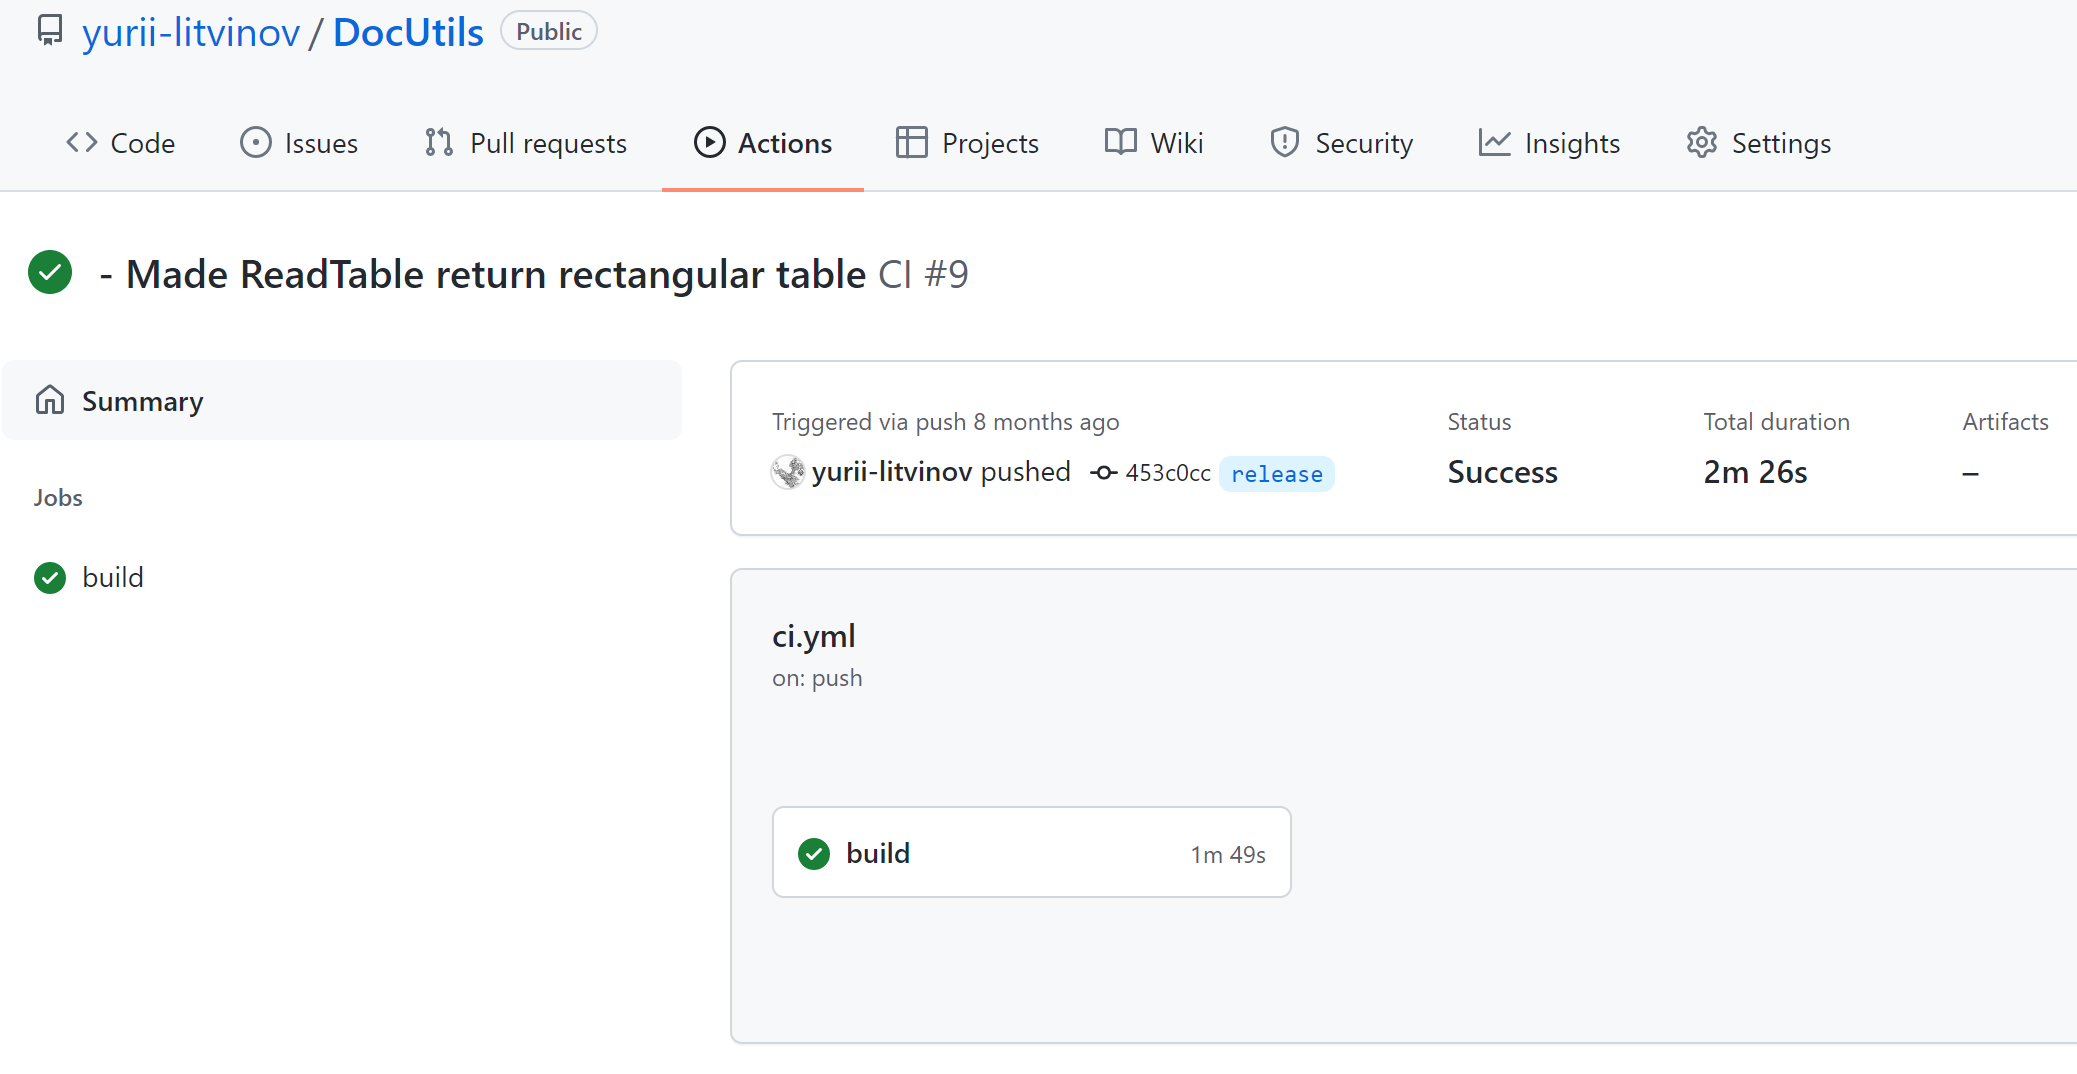
\includegraphics[width=0.9\textwidth]{githubActionsBuildStatus}
        \end{center}
        И появятся иконки статуса рядом с коммитами и пуллреквестами
    \end{frame}

    \begin{frame}[fragile]
        \frametitle{Типичный Workflow для сборки}
        \begin{scriptsize}
            \begin{minted}{yaml}
name: Build
on: [push, pull_request]
jobs:
    build-Ubuntu:
        runs-on: ubuntu-latest
        steps:
            - uses: actions/checkout@v2
            - uses: actions/setup-dotnet@v1
              with:
                  dotnet-version: '6.x'
            - name: Build
              run: For /R %%I in (*.sln) do dotnet build %%I
            - name: Run tests
              run: For /R %%I in (*.sln) do dotnet test %%I
    build-Windows:
        runs-on: windows-latest
        steps:
            ...
            - name: Build
              run: For /R %%I in (*.sln) do dotnet build %%I
            - name: Run tests
              run: For /R %%I in (*.sln) do dotnet test %%I
            \end{minted}
        \end{scriptsize}
    \end{frame}

    \begin{frame}
        \frametitle{GitHub Actions, Workflow и Job}
        \begin{center}
            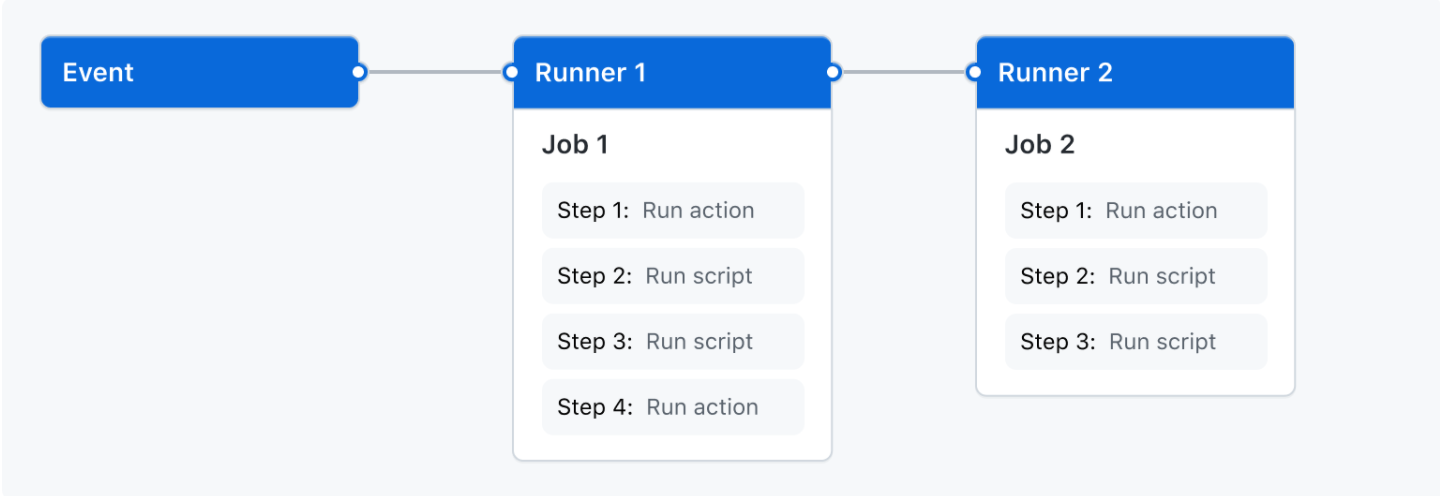
\includegraphics[width=0.7\textwidth]{githubActionsWorkflow}
        \end{center}
        \begin{itemize}
            \item Step --- это либо скрипт, либо \emph{Action}
            \item Action --- произвольный код (по сути, отдельное приложение), выполняющийся как шаг Job-а
            \begin{itemize}
                \item Переиспользуемый строительный блок
                \item Можно переиспользовать Workflow-ы
            \end{itemize}
        \end{itemize}
    \end{frame}

    \begin{frame}[fragile]
        \frametitle{Переменные окружения}
        \begin{scriptsize}
            \begin{minted}{yaml}
env:
  DAY_OF_WEEK: Monday

jobs:
  greeting_job:
    runs-on: ubuntu-latest
    env:
      Greeting: Hello
    steps:
      - name: "Say Hello Mona it's Monday"
        if: ${{ env.DAY_OF_WEEK == 'Monday' }}
        run: echo "$Greeting $First_Name. Today is $DAY_OF_WEEK!"
        env:
          First_Name: Mona
            \end{minted}
        \end{scriptsize}
    \end{frame}

    \begin{frame}[fragile]
        \frametitle{Матрица сборки}
        \begin{scriptsize}
            \begin{minted}{yaml}
runs-on: ${{ matrix.os }}
strategy:
  matrix:
    os: [ubuntu-18.04, ubuntu-20.04]
    node: [10, 12, 14]
steps:
  - uses: actions/setup-node@v2
    with:
      node-version: ${{ matrix.node }}
            \end{minted}
        \end{scriptsize}
    \end{frame}

    \begin{frame}
        \frametitle{Что ещё?}
        \begin{itemize}
            \item Секреты
            \begin{itemize}
                \item \mintinline{yaml}|super_secret: ${{ secrets.SUPERSECRET }}|
            \end{itemize}
            \item Кеширование промежуточных результатов
            \item Автоматическое развёртывание
            \begin{itemize}
                \item В том числе, автодеплой документации на github-pages
            \end{itemize}
            \item Проверка стиля кодирования, статический анализ кода и т.п.
            \begin{itemize}
                \item Может быть интересно для Python-разработчиков
            \end{itemize}
            \item Можно иметь несколько Workflow-ов в одном репозитории
        \end{itemize}
    \end{frame}

    \subsection{AppVeyor}

    \begin{frame}
        \frametitle{AppVeyor}
        \begin{itemize}
            \item \url{https://www.appveyor.com/} --- отдельная облачная CI-cистема, тоже довольно неплоха и проще в настройке
            \item Виртуальная машина с ОС Windows и настроенными инструментами сборки .NET-приложений
            \begin{itemize}
                \item Windows Server 2019 + VS 2022 или более старые
                \item Умеет Linux Ubuntu 20.04 и macOS 12.2.1
            \end{itemize}
            \item Интегрируется с GitHub-ом, Slack-ом, умеет деплоить
            \item Собирает по умолчанию системой сборки MSBuild
            \begin{itemize}
                \item Можно переубедить и собирать хоть C++-приложения
            \end{itemize}
            \item Окружение настраивается конфигурационным файлом или <<вручную>> из скрипта сборки
        \end{itemize}
    \end{frame}

    \begin{frame}
        \frametitle{AppVeyor, настройка сборки}
        \begin{itemize}
            \item Зайти на \url{https://www.appveyor.com/} по GitHub-аккаунту
            \item Добавить проект (разрешив AppVeyor просматривать список репозиториев на гитхабе)
            \item Положить в корень репозитория файл appveyor.yml с конфигурацией сборки
            \begin{itemize}
                \item Пустой тоже ок, это конфигурация по умолчанию, ищет .sln в корне репозитория и пытается его собрать
            \end{itemize}
            \item Закоммитить и запушить, это инициирует процесс сборки
            \item Результаты будут видны прямо на гитхабе, у каждого коммита и в пуллреквесте:
        \end{itemize}
        \begin{center}
            
\includegraphics[width=0.7\textwidth]{appVeyorSuccess.png}
        \end{center}
    \end{frame}

    \begin{frame}[fragile]
        \frametitle{AppVeyor, пример файла конфигурации}
        \begin{minted}{yaml}
image: Visual Studio 2022

before_build: 
    - nuget restore myCoolHomework/Homework.sln

build: 
    project: myCoolHomework/Homework.sln

test_script: 
    - dotnet test myCoolHomework/Homework.sln
        \end{minted}
    \end{frame}

    \section{CodeCov}

    \begin{frame}
        \frametitle{Анализ тестового покрытия, CodeCov}
        \begin{itemize}
            \item \url{https://codecov.io/}
            \item Визуализатор для функциональности компиляторов или специальных инструментов по слежению за исполнявшимися строчками
            \item Чем больше операторов было исполнено во время тестового прогона, тем меньше вероятность пропустить баг
            \begin{itemize}
                \item 100\% покрытие не гарантирует работоспособность программы
            \end{itemize}
            \item Интегрируется с GitHub (комментит пуллреквесты информацией о тестовом покрытии)
            \item Пример конфигурации для .NET с AppVeyor:
            \begin{itemize}
                \item \url{https://github.com/codecov/example-csharp}
            \end{itemize}
        \end{itemize}
    \end{frame}

    \section{Codacy}

    \begin{frame}
        \frametitle{Статический анализ, Codacy}
        \begin{itemize}
            \item \url{https://www.codacy.com/}
            \item Ищет типичные ошибки: потенциальные баги, стайлгайд, мёртвый код, производительность и т.д.
            \item Поддерживает много языков (в том числе C\#, C++, Java, Kotlin, Python, Scala)
            \item Не требует дополнительных манипуляций с репозиторием
            \item Очень настраиваема
        \end{itemize}
    \end{frame}

    \section{Trello}

    \begin{frame}
        \frametitle{Инструменты планирования, Trello}
        \begin{itemize}
            \item \url{https://trello.com/}
            \item Интерактивная доска с карточками, организованными в списки
            \item Карточки легко редактируются и перетаскиваются между списками
            \begin{itemize}
                \item Типичные списки: TODO, In Progress, Done (возможны варианты)
            \end{itemize}
            \item Поддерживает дедлайны, чеклисты, вложения, комментарии, голосования, метки
            \item Легковесный инструмент планирования, подходящий, тем не менее, и для больших проектов
        \end{itemize}
    \end{frame}

    \section{Pivotal Tracker}

    \begin{frame}
        \frametitle{Инструменты планирования, Pivotal Tracker}
        \begin{itemize}
            \item \url{https://www.pivotaltracker.com}
            \item Более ``тяжеловесный'' инструмент, ориентированный на Scrum
            \item Всего три списка
            \begin{itemize}
                \item Icebox --- что было бы неплохо сделать
                \item Backlog --- запланированные задачи
                \item Current --- задачи на текущую итерацию
            \end{itemize}
            \item Задачи можно оценивать, задачи имеют тип и статус
            \begin{itemize}
                \item По оценкам задач и статистике работы команды считается team velocity, позволяющая предсказать линейные сроки
            \end{itemize}
            \item Есть релизы с дедлайнами, метки, epic-и, чеклисты, вложения, комментарии
            \item Умеет считать статистику, рисовать графики (burndown charts)
        \end{itemize}
    \end{frame}

    \section{Slack и Gitter}

    \begin{frame}
        \frametitle{Средства коммуникации, Slack и Gitter}
        \begin{itemize}
            \item Instant messenger-ы, ориентированные на команды и интегрированные со средствами разработки
            \begin{itemize}
                \item Информация о коммитах и пуллреквестах
                \item Статус CI
                \item Другие тулы
            \end{itemize}
            \item Синтаксическая подсветка (markdown), вложения, отображение картинок, ...
            \item Gitter интегрирован с GitHub и ``более открыт'' (предназначается прежде всего для общения сообщества)
            \item Slack интегрирован с чем угодно, предназначается прежде всего для общения внутри команды
        \end{itemize}
    \end{frame}

    \section{GitHub}

    \begin{frame}
        \frametitle{GitHub: Issues, Projects, Wiki, Pages}
        \begin{itemize}
            \item GitHub сам многое умеет
            \item Issues --- довольно удобный багтрекер
            \begin{itemize}
                \item Майлстоуны, дедлайны, метки на багах, возможность закрывать баги автоматически (если в сообщении коммита есть ``close'' или ``fix'' и \#<номер бага>)
                \item Пуллреквест тоже считается Issue
            \end{itemize}
            \item Projects --- представляет Issues в виде набора списков, между которыми их можно перетаскивать в духе Trello
            \item Wiki --- викистраницы, куда можно выкладывать полезную информацию о проекте
            \begin{itemize}
                \item Тоже git-репозиторий
            \end{itemize}
            \item Pages --- хостинг для статических сайтов <имя проекта>.github.io
        \end{itemize}
    \end{frame}

    \section{Авторское право}

    \begin{frame}
        \frametitle{Авторское право}
        \begin{itemize}
            \item Open source-кодом можно пользоваться, только если автор явно это разрешил, так что просто код на GitHub --- не совсем open source
            \item Бывают исключительные и личные неимущественные права
            \begin{itemize}
                \item Личные неимущественные права неотчуждаемы
                \item Исключительные права можно передать
                \item Права появляются в момент создания произведения и принадлежат автору
                \begin{itemize}
                    \item Если произведение создано по служебному заданию --- работодателю
                    \item Знак копирайта служит только для информирования, регистрация прав не требуется
                \end{itemize}
                \item Соавторы владеют произведением в равной степени
            \end{itemize}
            \item Идея не охраняется, охраняется её физическое выражение
        \end{itemize}
    \end{frame}

    \begin{frame}
        \frametitle{Open source-лицензии}
        \begin{itemize}
            \item Лицензия --- способ передачи части прав на произведение
            \item Пример --- ``Do what the **** you want to public license''
            \begin{itemize}
                \item ``Want to'' может включать в себя патентование произведения и подачу в суд на автора за нарушение патента, поэтому обычно лицензии более длинны и унылы
                \item В России и Европе программы не патентуют, в США --- да
            \end{itemize}
            \item Каждый нормальный open source-проект должен иметь лицензию
        \end{itemize}
    \end{frame}

    \begin{frame}
        \frametitle{Open source-лицензии}
        \begin{itemize}
            \item Часто используемые open source-лицензии:
            \begin{itemize}
                \item GPL, LGPL (GPL вирусная, поэтому использовать её, внезапно, плохая практика)
                \item MIT License
                \item Apache License 2.0 (может применяться пофайлово)
                \item BSD License (в разных вариантах)
                \item The Unlicense --- явная передача произведения в Public Domain
                \item Семейство лицензий Creative Commons --- не для софта, но хорошо подходит для ресурсов (картинок, текстов и т.д.)
            \end{itemize}
        \end{itemize}
    \end{frame}

\end{document}
